\documentclass[letterpaper,twocolumn,amsmath,amssymb,pre]{revtex4-1}
\usepackage{graphicx}% Include figure files
\usepackage{dcolumn}% Align table columns on decimal point
\usepackage{bm}% bold math
\usepackage{color}
\usepackage{breqn}

\newcommand{\red}[1]{{\bf \color{red} #1}}
\newcommand{\blue}[1]{{\bf \color{blue} #1}}
\newcommand{\green}[1]{{\bf \color{green} #1}}
\newcommand{\rr}{\textbf{r}}
\newcommand{\refnote}{\red{[ref]}}

\newcommand{\fixme}[1]{\red{[#1]}}

%\newcommand{\derivation}[1]{#1} % Use this to show all derivations in detail
\newcommand{\derivation}[1]{} % Use this for nice pegagogical paper...

% needsworklater is used to annotate bits that need work, but that we
% can postpone for a while.
\newcommand{\needsworklater}[1]{\emph{[#1]}}
% needsworknow is intended to prioritize stuff that needs fixing.
\newcommand{\needsworknow}[1]{\textcolor{red}{[\emph{#1}]}}

\begin{document}
\title{E Coli project paper}

%\pacs{61.20.Ne, 61.20.Gy, 61.20.Ja}
%%%%%%%%%%%%%%%%%%%%%%%%%%%%%%%%%%%%%%%%%%%%%%%%%%%%%%%%%%%%
\begin{abstract}
  This paper is about science.
\end{abstract}

<<<<<<< HEAD
\section{Introduction}
\subsection{What is the MinD system and why is it important?}
-Systm of proteins in E.Coli and other cells.
-Theorized to be instrumental in cell citokenisis. Reference experiments
\subsection{How proteins move in cell}
-Reference experimental showing proteins oscillating
-Reference theory showing difEQ model shows oscillations
-Reference Mannik shoving into crevices.
-Worthwhile studying effect of walls shape on the movement of cells
(Sign post of what to expect from this paper)

\section{Methods and Initial Conditions}
\subsection{Mathematical Model} %shouldn't be a scripty mu
The model for the behavio r of the MinD and MinE proteins inside the cell
implemented the same set of 5 reaction-diffusion equations described in the paper
by Huang et al (equations 1, 2, 3, 4, and 5). A 3d grid was constructed in
cartesian coordinates with a grid spacing of .05 $\mu$m. From there, we
were able to define a cell shape on the grid, and solve the
reaction-diffusion equations numerically to observe the time evolution of
the MinD and MinE concentrations inside the cell.

Our simulation used the same diffusion constants and reaction rates as
Huang et al, which are

\begin{align*} %format better
  \mathcal{D}_D = \mathcal{D}_{E}  = 2.5 \mu \textrm{m$^2$ / sec}, \\
  \sigma_D^{\textrm{ADP $\rightarrow$ ATP}} = 1/\textrm{sec},  \sigma_D = 0.025 \mu \textrm{m/sec}, \\
  \sigma_{dD} = 0.0015 \mu \textrm{m$^3$/sec}, \\
  \sigma_{de} = 0.7/\textrm{sec}, \sigma_E = 0.093 \mu \textrm{$m^3$/sec}.
\end{align*}

To test our computational model, we implemented a pill shaped cell, and
tested using the same cell parameters as Huang et al, which were a radius
of 0.5 $\mu$m in the middle and at the spherical endcaps, and two different
cell lengths of 4 $\mu$m and 10 $\mu$m. We found the same type of
oscillations as in their paper using these initial conditions, verifying
that our model works as intended. Below are snapshots of MinD and MinE
concentrations at 5 second timestamps in the 4 $\mu$m cell:
\newline
\newline
[insert 5 second time stamps of 4 $\mu$m sim]
\newline
\newline
We then began to define other, non-traditional cell shapes for the purpose of
modeling squished and perturbed E. coli cells, which were created
experimentally in Mannick et al. To achieve this, we went with a
cartesian lattice rather than the cylindrical lattice used in Huang et 
al's simulations, as it allows for more flexibility in defining the 
cell shape. Some of the cell shape models included a flattened pill
(stadium shape), an ellipsoid, a spherical cell, and various randomly
generated smooth shapes, such as those in the figures below. 
\newline
\newline
[insert memf print of 2-3 cell shapes]
\newline
\newline
To interpret the results, we generated several different plot views of
the printed simulation data. These plots included a time averaged view
of the protein densities in the cell; a plot tracking the location of
protein concentrations that were global maxima in space and local maxima in 
time; and an animated view that showed the actual dispersion of
protein concentrations in the cell over time. 
\section{Specific Results}
-Datahjhuj and plots that show concrete results. Pill normal is for the establishing that we have what works, reference other paper, then modify, is the idea.
Pill Normal -

Pill Short -
     -Know how short is too short

Randst 99 -

\begin{figure}
  \includegraphics[width=\columnwidth]{../data/shape-randst/plots/time-map-compare-randst-10-60-60-990-150.pdf}
  \caption{randst 99}
  %\label{}
\end{figure}
\begin{figure}
  \includegraphics[width=\columnwidth]{../data/shape-randst/plots/time-map-compare-randst-10-80-60-980-150.pdf}
  \caption{randst 98}
  %\label{fig:pair-distribution-3}
\end{figure}
\begin{figure}
  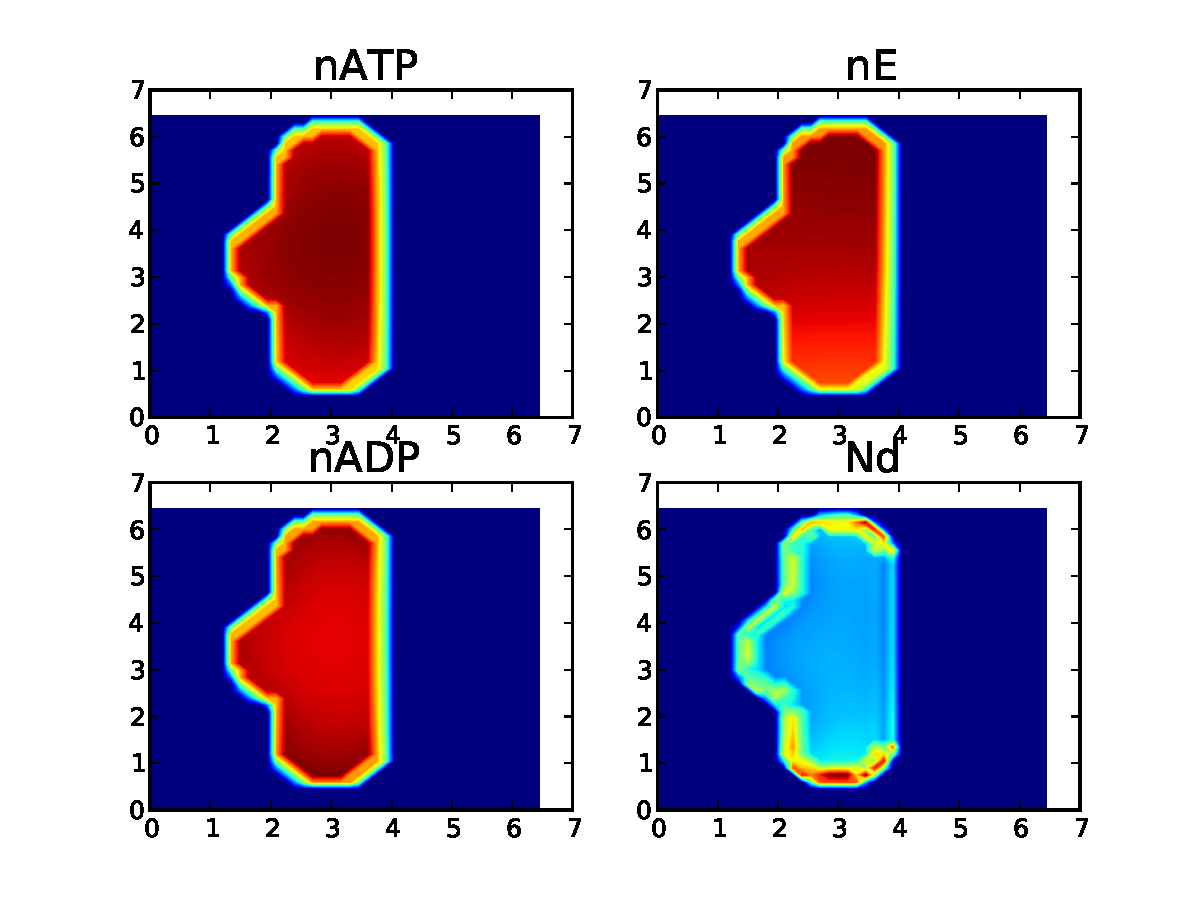
\includegraphics[width=\columnwidth]{../data/shape-randst/plots/time-map-compare-randst-10-60-60-970-150.pdf}
  \caption{randst 97}
  %\label{fig:pair-distribution-3}
\end{figure}
\begin{figure}
  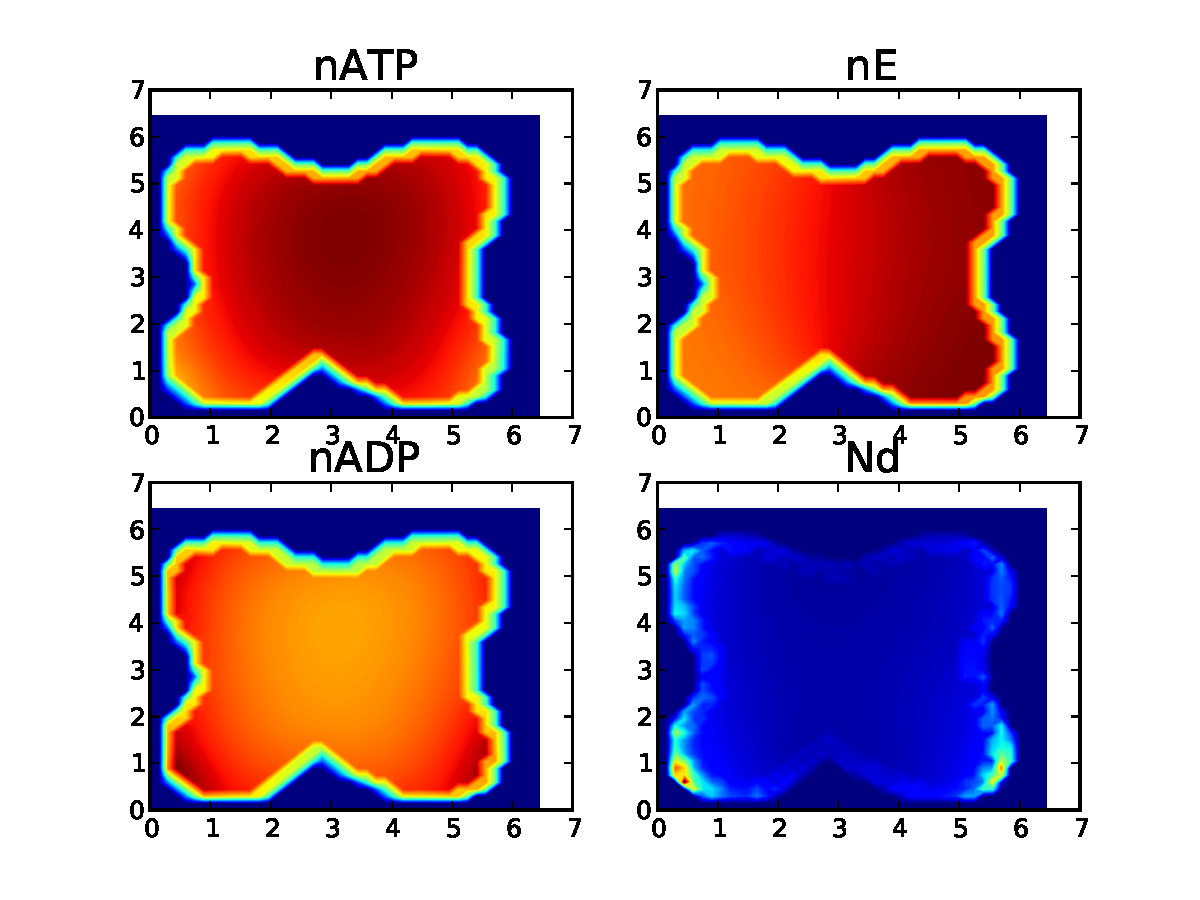
\includegraphics[width=\columnwidth]{../data/shape-randst/plots/time-map-compare-randst-10-60-60-960-150.pdf}
  \caption{randst 96}
  %\label{fig:pair-distribution-3}
\end{figure}

Randst 98 -

Randst 97 -

Randst 96 -

Triangle -


\section{Interpretation of Data}
-Discussion of conceptual reasons of why we see what we see
-Plots that are more interpretive (area-rating)
-Some sort of predictive claim?


\section{Conclusion}


\appendix

\section*{Appendix}


\end{document}
